\documentclass[10pt,a4paper]{article}
\usepackage[utf8]{inputenc}
\usepackage[english]{babel}
\usepackage{amsmath}
\usepackage{amsfonts}
\usepackage{amssymb}
\usepackage{makeidx}
\usepackage{graphicx}
\usepackage{fourier}
\usepackage{hyperref}
\usepackage[left=2cm,right=2cm,top=2cm,bottom=2cm]{geometry}
\author{Miguel Molinos Pérez}
\title{MPM}
\begin{document}


\title{Notes about the Generalized Interpolation Material Point
  Method} \author{
  Miguel Molinos P\'erez\\ \\
  \small{Dpto. de Matem\'aticas Aplicadas}\\
  \small{Universidad Polit\'ecnica de Madrid (UPM)}\\
  \small{\texttt{m.molinos@alumnos.upm.es}} } \date{\small{\today}}


\maketitle % Titulo
\newpage
\tableofcontents
% Idndice de contenidos

% Introduction

\section{Introduction}
\label{sec:intro}

The past several decades have brought tremendous advances in computing
power and provided fertile ground for the development of the
computational sciences. In computational solid mechanics the Finite
Element Method (FEM) (METER CITA MOLONA) has been very successfully
applied to a wide range of problems with good results. However, body
fixed FEM meshes can be difficult and time consuming to generate for
complex three-dimensional objects. Further, mesh distorsion associated
with large deformations compromises solution accuracy, ultimately
requiring re-meshing. These difficulties have spurred the development
of alternative discretization strategies which avoid mesh distorsion by
dicretizing at points and never
maintaining a body-fixed mesh.\\

Quite a number of ''meshless methods'' have been developed. Some of
the ways in which the methods differ include whether or not a
temporary mesh is used in the solution procedure, whether the
discretization procedure begins with the

\cite{Schreyer1994}


%%% Local Variables:
%%% mode: latex
%%% TeX-master: "../../../mpm"
%%% End:


% Derivation of discrete Equations

\section{Governing Equations}
\label{sec:deriv_eq}

In  the following  derivation  of the  discrete  equations, bold  face
quantities  indicate tensor,  $\nabla$ id  the gradient  operator, and
$\cdot$,  and $:$  are first  order (vector)  and second  order tensor
contraction, respectively. The subscript $p$ is used to index material
point  variables   and  $i$   grid  vertex  variables.   The  notation
$\sum_p^{Np}$ and $\sum_i^{Np}$  is used to denote  summation over all
material points, and over all grid vertex, respectively.\\

Of  interest  in  solid  mechanics is  the  deformation  and  material
response to a continuous solid  body under prescribed loads and initial
conditions,    as   governed    by    conservation    of   mass    and
momentum.  Conservation of  mass  is satisfied  implicitly by  leaving
discrete particle  masses unchanged throughout a  computation. Here we
develop  the  discrete  version  of conservation  of  momentum,  which
permits  evolution  of  particle  momenta   in  time.  We  consider  a
deformable body acted upon by forces and subjected to either kinematic
or  traction  boundary conditions  every  where  on its  surface.  The
continuum mechanics theory

\begin{itemize}
\item Balance of momentum
\item Compatibility
\item
\end{itemize}

 
We works over the balance of momentum in the strong formulation, as we
can see in \ref{eq:sf_conserv_momentum}

\begin{equation}
  \label{eq:sf_conserv_momentum}
  \rho a = \nabla \cdot(\sigma) + \rho b  
\end{equation}

Multiplying (\ref{eq:sf_conserv_momentum}) by $\psi$ we get
(\ref{eq:sf_conserv_momentum_2})

\begin{equation}
  \label{eq:sf_conserv_momentum_2}
  \psi^T \cdot \rho a = \psi^T \cdot \nabla\cdot(\sigma) + \psi^T \cdot \rho b
\end{equation}

The function $\psi$ belongs to a space $\mathcal{H}$ (vectorial space
with scalar product defined) wich verifies
$a(\ddot{u},\dot{u},u,\psi)=l(\psi) \quad \forall\ \psi\ \in\
\mathcal{H}$. In other hand, in every point of $\Omega$ where we have
imposed the Dirichlet bounday condition,


\begin{equation}
  \label{eq:hilbert_space}
  \mathcal{H} = \{  \psi(x)/\psi \mid_{\Gamma_D} = 0 \quad , \quad \psi \in H^1(\Omega)  \}
\end{equation}

In other words, $\mathcal{H}$ is the space defined by all the
functions $g$, that $ \psi$ and $\nabla \psi$ are FUNCIONES DE
CUADRADO INTEGRABLE in $\Omega$

\begin{equation}
  \label{eq:def_psi}
  \int_{\Omega}\psi\ d\Omega < \infty \quad , \quad \int_{\Omega}\nabla\psi\ d\Omega < \infty
\end{equation}

Integrating (\ref{eq:sf_conserv_momentum_2}) over $\Omega$ we get
(\ref{eq:wf_conserv_momentum_1})

\begin{equation}
  \label{eq:wf_conserv_momentum_1}
  \int_{\Omega} \psi^T \cdot \rho a\ d\Omega = \int_{\Omega} \psi^T \cdot \nabla\cdot(\sigma)\ d\Omega + \int_{\Omega} \psi^T \cdot \rho b\ d\Omega
\end{equation}

integrating by parts the therm of the internal tension in
(\ref{eq:wf_conserv_momentum_1}), we get (\ref{eq:wf_conserv_momentum_2})

\begin{equation}
  \label{eq:wf_conserv_momentum_2}
  \int_{\Omega} \psi^T\cdot \rho a\ d\Omega = \int_{\Omega}  \nabla\cdot \left( \psi^T \cdot
    \sigma \right)\ d\Omega - \int_{\Omega}  \nabla\psi^T : \sigma\ d\Omega
  + \int_{\Omega} \psi^T\cdot b\ d\Omega
\end{equation}

applying the Gauss theorem over (\ref{eq:wf_conserv_momentum_2}), and following the definition of the stress
vector $t = \sigma \cdot n$ where $n$ is the vector orthogonal to a
surface in the solid, finally we get the variational form for
conservation of momentum may be written as
\ref{eq:wf_conserv_momentum3}

\begin{equation}
  \label{eq:wf_conserv_momentum3}
  \int_{\Omega} \psi^T \cdot \rho a\ d\Omega = \int_{\Gamma}  \psi^T
  \cdot \overbrace{\sigma \cdot n}^{t}\ d\Gamma - \int_{\Omega}  \nabla \psi^T : \sigma\ d\Omega
  + \int_{\Omega} \psi^T b\ d\Omega  
\end{equation}


% \subsection{Initial discretization}
% \label{sec:ini_discr}

% The particle characteristic function are required to be a partition of
% unity in the initial configuration as we can see in
% (\ref{eq:part_uniti_chi_i}).

% \begin{equation}
%   \label{eq:part_uniti_chi_i}
%   \sum_{p=1}^{Np}\chi_p^i(x)\ =\ 1
% \end{equation}

% Where $\chi_p^i$ denotes the particle characteristic functions
% restricted to their initial positions and undeformed state. In the
% simplest cases, particle characteristic function are taken to be
% initially non-overlapping. However, nothing precludes overlapping, or
% ''fuzzy'' particles, as discussed later. Initial particle volumes
% $V_p^i$ are defined by (\ref{eq:vpi_def}).
% \begin{equation}
%   \label{eq:vpi_def}
%   V_p^i = \int_{\Omega^i}\chi^i_p(x)\ d\Omega
% \end{equation}
% where $\Omega^i$ is the initial volume of the continuum body to be
% discredited. In addition to initial particle volumes, the material
% point initial masses, $m_p^i$, momenta, $p_p^i$ ans stresses,
% $\sigma_p^i$, must be defined. These properties of the continuum
% against the particle characteristic functions, as we can see in the
% equations (\ref{eq:m_pi}) and (\ref{eq:p_pi})

% \begin{align}
%   \label{eq:m_pi}
%   m_p^i =& \int_{\Omega_i}\rho^i(x)\chi_p^i(x)\ d\Omega \\
%   \label{eq:p_pi}
%   p_p^i =& \int_{\Omega_i}\rho^i(x)v^i(x)\chi_p^i(x)\ d\Omega
% \end{align}

% where $\rho^i$

% \subsection{Discrete Solution Procedure}
% \label{sec:discr_sol_proc}

% Given a material point property, $f_p$, a representation consistent
% with the initial discretization procedure is the sum over the material
% points.
% \begin{equation}
%   \label{eq:mat_point_discretiz}
%   f(x) = \sum_p^{Np}f_p \chi_p(x)  
% \end{equation}

% The particle characteristic functions are used as a basis for
% representing particle data throughout the computational domain and
% determine the degree of smoothness of the spatial variation.

% Approaching term by term of (\ref{eq:wf_conserv_momentum3}) using
% (\ref{eq:mat_point_discretiz}) we get the following :



% \begin{itemize}
% \item Acceleration term :
%   \begin{eqnarray}
%     \label{eq:wf_conserv_momentum_acc}
%    \int_{\Omega} \psi^T \rho \cdot a \cdot d\Omega =& \int_{\Omega} \psi^T \frac{m}{V}
%                                                      \dot{v}\ d\Omega = \int_{\Omega} \psi^T \frac{1}{V}
%                                                      \overbrace{m\dot{v}}^{\dot{p}}\ d\Omega = \int_{\Omega} \psi^T \frac{\dot{p}}{V} d\Omega = \nonumber \\
%   =&  \int_{\Omega} \psi^T \left[ \sum^{Np}_{p=1} \frac{\dot{p}_p}{V_p} \chi_p(x) \right]\ d\Omega =
%      \sum^{Np}_{p=1} \left[ \int_{\Omega_p \bigcap \Omega}
%      \psi^T\frac{\dot{p}_p}{V_p}\chi_p(x)\ d\Omega \right] 
%   \end{eqnarray}


% \item Internal forces :
%   \begin{align}
%     \label{eq:wf_conserv_momentum_int_forces}
%     \int_{\Omega}  \nabla \psi^T \sigma\ d\Omega = \int_{\Omega}  \nabla
%     \psi^T \left[\sum^{Np}_{p=1} \sigma_p \chi_p(x) \right]\ d\Omega =
%     \sum^{Np}_{p=1} \left[ \int_{\Omega_p \bigcap \Omega}
%     \nabla\psi^T\sigma_p\chi_p(x)\ d\Omega \right]
%   \end{align}
% \item External forces :
%   \begin{align}
%     \label{eq:wf_conserv_momentum_ext_forces}
%     \int_{\Omega} \psi^T \rho b\ d\Omega =& \int_{\Omega} \psi^T \frac{m}{V} b\
%                                            d\Omega = \int_{\Omega} \psi^T \left[ \sum^{Np}_{p=1}
%                                            \frac{m_p}{V_p}\chi_p(x) \right] b\ d\Omega = \sum_{p=1}^{Np}
%                                            \left[ \int_{\Omega_p \bigcap \Omega}
%                                            \psi^T \frac{m_p}{V_p} \chi_p(x) b\ d\Omega \right]
%   \end{align}  
% \end{itemize}

% Finally we get the \eqref{eq:sf_conserv_momentum} with the GIPM
% discretization as \eqref{eq:wf_conserv_momentum_GIMP}:

% \begin{align}
%   \label{eq:wf_conserv_momentum_GIMP}
%   \sum^{Np}_{p=1} \left[  \int_{\Omega_p \bigcap \Omega}
%   \psi^T\frac{\dot{p}_p}{V_p}\chi_p(x)\ d\Omega \right] + \sum^{Np}_{p=1} \left[ \int_{\Omega_p \bigcap \Omega}
%   \nabla\psi^T\sigma_p\chi_p(x)\ d\Omega \right] =
%   \int_{\Gamma}\psi^T t\ d\Gamma + \sum_{p=1}^{Np}
%   \left[ \int_{\Omega_p \bigcap \Omega}
%   \psi^T \frac{m_p}{V_p} \chi_p(x) b\ d\Omega \right]
% \end{align}
% \\
% where $\Omega_p$ denotes the current support of particle
% characteristic function p, and the current particle volumes are
% defined by (\ref{eq:charact_volum})

% \begin{equation}
%   \label{eq:charact_volum}
%   V_p = \int_{\Omega_p \bigcap \Omega} \chi_p(x)\ d\Omega
% \end{equation}

% Rewriting the balance of momentum, the equation 


% The other fundamental aspect of PIC methods is the use of a
% computational grid. In MPM the grid serves as a scratch pad for the
% solution of conservation of momentum, from which particle states are
% updated. To complete the discretization procedure, approximations to
% the admissible velocity fields, or test functions, are introduced in
% terms of grid vertex quantities and grid shape functions. This step is
% analogous to the development of FEM discrete equations. However, use
% of both grid and particle basis functions to represent test functions
% and trial functions, respectively, is a Petrov–Galerkin method,
% [Johnson (1987)], and therefore more akin to some of the meshless
% methods (in particular [Demkowicz and Oden (1986); Atluri and Zhu
% (2000)]) than the FEM. The continuous representation, $g(x)$, of grid
% data, $g_i$ , then
% \begin{equation}
%   g(x) = \sum_{i = 1}^{Nn}=g_iN_i(x)
% \end{equation}

% Here $N_i(x)$ is a computational grid shape function, which takes unit
% value at node $i$ and zero value all the other nodes. Further, the
% shape function are required to be a partition of unity

% \begin{equation}
%   \label{eq:Partition_Unity}
%   \sum_{i=1}^{Nn} N_i(x) = 1  
% \end{equation}


% \begin{eqnarray}  
%   \sum^{Np}_{p=1} \left[ \int_{\Omega_p \bigcap \Omega}
%   \psi^T\frac{\dot{p}_p}{V_p}\chi_p(x) d\Omega \right] =& \sum^{Np}_{p=1}\left[ \frac{1}{V_p}\int_{\Omega_p \bigcap \Omega} N_i(x) \chi_p(x) d\Omega \dot{p}_p  \right] = \nonumber \\
%   =& \sum_{p=1}^{Np} \overline{S}_{ip}\cdot \dot{p}_p = \dot{p}_i
% \end{eqnarray}

% \begin{eqnarray}
%   -\sum^{Np}_{p=1}\left[ \int_{\Omega_p \bigcap \Omega}\nabla\psi^T \sigma_p \chi_p  d\Omega \right] =& -\sum^{Np}_{p=1}\left[ \int_{\Omega_p \bigcap \Omega}\nabla N_i(x) \sigma_p \chi_p  d\Omega \right] = \nonumber \\
%   =& - \sum^{Np}_{p=1}\left[ \frac{V_p}{V_p} \int_{\Omega_p \bigcap \Omega}\nabla N_i(x) \chi_p  d\Omega \sigma_p \right] = \nonumber \\
%   =& - \sum^{Np}_{p=1}\left[V_p\overline{\nabla S}_{ip} \sigma_p \right] = f_i^{int}
% \end{eqnarray}

% \begin{equation}
%   \int_{\Gamma \equiv \partial \Omega} \psi^T t d\Gamma = \int_{\Gamma \equiv \partial \Omega} N_i(x) t d\Gamma = f_i^t
% \end{equation}

% \begin{eqnarray}
%   \sum_{p=1}^{Np} \left[ \int_{\Omega_p \bigcap \Omega} \psi^T \frac{m_p}{V_p} \chi_p(x) b d\Omega \right] = \sum_{p=1}^{Np} \left[ \int_{\Omega_p \bigcap \Omega} N_i(x)  \frac{m_p}{V_p} \chi_p(x) b d\Omega  \right] =  \sum_{p=1}^{Np} \overline{S}_{ip}b m_p = f_i^b  
% \end{eqnarray}


% \begin{eqnarray}
%   \sum_{p=1}^{Np} \overline{S}_{ip}\cdot \dot{p}_p  =
%   -\sum^{Np}_{p=1}\left[V_p\overline{\nabla S}_{ip} \sigma_p \right]
%   +&  \int_{\Gamma \equiv \partial \Omega} N_i(x) t d\Gamma \nonumber
%      +& \sum_{p=1}^{Np} \overline{S}_{ip}b m_p \nonumber\\
%   \Downarrow&  \\
%   \dot{p}_p = f_i^{int} + f_i^t + f_i^b \nonumber
% \end{eqnarray}





\subsection{Observations}
\label{sec:observations}




%%% Local Variables:
%%% mode: latex
%%% TeX-master: "../../../mpm"
%%% End:


% The state of art of the MPM

\section{State of art of the material point method}
\label{sec:state-art-material}

The material point method (MPM) was developed by Sulsky and coworkers,
see \cite{Schreyer1994}, as an extension for solids mechanics of the
fluid-implicit particle-method (FLIP) developed by (Brackbill). Further, the
FLIP originally was proposed as an extension of the particle-in-cell
method developed by (Harlow). More recent developments are centered in
trying to solve the well-know grid-crossing error of the MPM,
described deeply in \ref{sec:grid-crossing-errors}, the first of this early attempts was the
presented by \cite{Bardenhagen2004} called the generalized interpolation
material point method (GIMP), other approach to solve this problem are
the implicit Generalized Interpolation Material Point (GIMP) presented
by \cite{Charlton2017}, the convected Particle Domain Interpolation
(CPDI) and the second-order convected particle domain interpolation
(CPDI 2) by \cite{Sadeghirad2013}, \cite{Sadeghirad2013a}, the dual
Domain Material Point Method (DDMPM) by \cite{Zhang2011}, and the
B-Spline MPM by \cite{Bing2019}.

All of this methods has a starting point the variation form for
conservation momentum \eqref{eq:wf_conserv_momentum3} presented in
\ref{sec:deriv_eq}. In order to arrive to a finite set of equations,
the continuum domain $\Omega$ is discretized as as a finite sum of
material points. Here, the index $p$ is used for the material point
values, $I$ for the nodes of the grid nodes and the index $i,j,k$ are
used for the dimensions of the variables. Each material point has a
position $x_{p,i}$ defined by the centroid of the volume $\Omega_p$.

Each material point is assigned initial values of position, velocity,
mass, volume and stress, denoted by $x_{p,i}$, $v_{p,i}$, $m_{p}$, $V_{p,i}$,
$\sigma_{p,ij}$, and others. Given a material point property, $f_p$, a
representation consistent with the initial discretization procedure is
the sum over the material point as we can see in \eqref{eq:mpm_discretization}
\begin{equation}
  \label{eq:mpm_discretization}
  f(x_i,t) = \sum_p^{N_p} f_p(t) \chi_p(x_i)
\end{equation}
where $\chi$ denotes the particle characteristic function.

As an example, the density field can be discretized as we can see in
\eqref{eq:mpm_density}.
\begin{equation}
  \label{eq:mpm_density}
  \rho(x_i,t) =  \sum_p^{N_p}m_p \chi_p(x_i)
\end{equation}
In order to discretize the stress therm of  \eqref{eq:wf_conserv_momentum3}, a specific
stress is defined by \eqref{eq:specific_stress}
\begin{equation}
  \label{eq:specific_stress}
  \sigma_s = \frac{\sigma}{rho}
\end{equation}
so the stress term becomes
\begin{equation}
  \label{eq:specific_stress_intforces}
  \int_{\Omega}  \nabla \psi^T : \sigma\ d\Omega = \int_{\Omega}  \nabla \psi^T : \rho\sigma_s\ d\Omega
\end{equation}

\subsection{The original material point method}
\label{sec:orig-mater-point}

The particle characteristic function are required to be a partition of
unity in the initial configuration as we can see in
(\ref{eq:part_uniti_chi_i}).

\begin{equation}
  \label{eq:part_uniti_chi_i}
  \sum_{p=1}^{Np}\chi_p^i(x)\ =\ 1
\end{equation}

Where $\chi_p^i$ denotes the particle characteristic functions
restricted to their initial positions and undeformed state. In the
simplest cases, particle characteristic function are taken to be
initially non-overlapping. However, nothing precludes overlapping, or
''fuzzy'' particles, as discussed later. Initial particle volumes
$V_p^i$ are defined by (\ref{eq:vpi_def}).
\begin{equation}
  \label{eq:vpi_def}
  V_p^i = \int_{\Omega^i}\chi^i_p(x)\ d\Omega
\end{equation}
where $\Omega^i$ is the initial volume of the continuum body to be
discredited. In addition to initial particle volumes, the material
point initial masses, $m_p^i$, momenta, $p_p^i$ ans stresses,
$\sigma_p^i$, must be defined. These properties of the continuum
against the particle characteristic functions, as we can see in the
equations (\ref{eq:m_pi}) and (\ref{eq:p_pi})

\begin{align}
  \label{eq:m_pi}
  m_p^i =& \int_{\Omega_i}\rho^i(x)\chi_p^i(x)\ d\Omega \\
  \label{eq:p_pi}
  p_p^i =& \int_{\Omega_i}\rho^i(x)v^i(x)\chi_p^i(x)\ d\Omega
\end{align}

where $\rho^i$

\subsection{Discrete Solution Procedure}
\label{sec:discr_sol_proc}

Given a material point property, $f_p$, a representation consistent
with the initial discretization procedure is the sum over the material
points.
\begin{equation}
  \label{eq:mat_point_discretiz}
  f(x) = \sum_p^{Np}f_p \chi_p(x)  
\end{equation}

The particle characteristic functions are used as a basis for
representing particle data throughout the computational domain and
determine the degree of smoothness of the spatial variation.

Approaching term by term of (\ref{eq:wf_conserv_momentum3}) using
(\ref{eq:mat_point_discretiz}) we get the following :



\begin{itemize}
\item Acceleration term :
  \begin{eqnarray}
    \label{eq:wf_conserv_momentum_acc}
   \int_{\Omega} \psi^T \rho \cdot a \cdot d\Omega =& \int_{\Omega} \psi^T \frac{m}{V}
                                                     \dot{v}\ d\Omega = \int_{\Omega} \psi^T \frac{1}{V}
                                                     \overbrace{m\dot{v}}^{\dot{p}}\ d\Omega = \int_{\Omega} \psi^T \frac{\dot{p}}{V} d\Omega = \nonumber \\
  =&  \int_{\Omega} \psi^T \left[ \sum^{Np}_{p=1} \frac{\dot{p}_p}{V_p} \chi_p(x) \right]\ d\Omega =
     \sum^{Np}_{p=1} \left[ \int_{\Omega_p \bigcap \Omega}
     \psi^T\frac{\dot{p}_p}{V_p}\chi_p(x)\ d\Omega \right] 
  \end{eqnarray}


\item Internal forces :
  \begin{align}
    \label{eq:wf_conserv_momentum_int_forces}
    \int_{\Omega}  \nabla \psi^T \sigma\ d\Omega = \int_{\Omega}  \nabla
    \psi^T \left[\sum^{Np}_{p=1} \sigma_p \chi_p(x) \right]\ d\Omega =
    \sum^{Np}_{p=1} \left[ \int_{\Omega_p \bigcap \Omega}
    \nabla\psi^T\sigma_p\chi_p(x)\ d\Omega \right]
  \end{align}
\item External forces :
  \begin{align}
    \label{eq:wf_conserv_momentum_ext_forces}
    \int_{\Omega} \psi^T \rho b\ d\Omega =& \int_{\Omega} \psi^T \frac{m}{V} b\
                                           d\Omega = \int_{\Omega} \psi^T \left[ \sum^{Np}_{p=1}
                                           \frac{m_p}{V_p}\chi_p(x) \right] b\ d\Omega = \sum_{p=1}^{Np}
                                           \left[ \int_{\Omega_p \bigcap \Omega}
                                           \psi^T \frac{m_p}{V_p} \chi_p(x) b\ d\Omega \right]
  \end{align}  
\end{itemize}

Finally we get the \eqref{eq:sf_conserv_momentum} with the GIPM
discretization as \eqref{eq:wf_conserv_momentum_GIMP}:

\begin{align}
  \label{eq:wf_conserv_momentum_GIMP}
  \sum^{Np}_{p=1} \left[  \int_{\Omega_p \bigcap \Omega}
  \psi^T\frac{\dot{p}_p}{V_p}\chi_p(x)\ d\Omega \right] + \sum^{Np}_{p=1} \left[ \int_{\Omega_p \bigcap \Omega}
  \nabla\psi^T\sigma_p\chi_p(x)\ d\Omega \right] =
  \int_{\Gamma}\psi^T t\ d\Gamma + \sum_{p=1}^{Np}
  \left[ \int_{\Omega_p \bigcap \Omega}
  \psi^T \frac{m_p}{V_p} \chi_p(x) b\ d\Omega \right]
\end{align}
\\
where $\Omega_p$ denotes the current support of particle
characteristic function p, and the current particle volumes are
defined by (\ref{eq:charact_volum})

\begin{equation}
  \label{eq:charact_volum}
  V_p = \int_{\Omega_p \bigcap \Omega} \chi_p(x)\ d\Omega
\end{equation}

Rewriting the balance of momentum, the equation 


The other fundamental aspect of PIC methods is the use of a
computational grid. In MPM the grid serves as a scratch pad for the
solution of conservation of momentum, from which particle states are
updated. To complete the discretization procedure, approximations to
the admissible velocity fields, or test functions, are introduced in
terms of grid vertex quantities and grid shape functions. This step is
analogous to the development of FEM discrete equations. However, use
of both grid and particle basis functions to represent test functions
and trial functions, respectively, is a Petrov–Galerkin method,
[Johnson (1987)], and therefore more akin to some of the meshless
methods (in particular [Demkowicz and Oden (1986); Atluri and Zhu
(2000)]) than the FEM. The continuous representation, $g(x)$, of grid
data, $g_i$ , then
\begin{equation}
  g(x) = \sum_{i = 1}^{Nn}=g_iN_i(x)
\end{equation}

Here $N_i(x)$ is a computational grid shape function, which takes unit
value at node $i$ and zero value all the other nodes. Further, the
shape function are required to be a partition of unity

\begin{equation}
  \label{eq:Partition_Unity}
  \sum_{i=1}^{Nn} N_i(x) = 1  
\end{equation}


\begin{eqnarray}  
  \sum^{Np}_{p=1} \left[ \int_{\Omega_p \bigcap \Omega}
  \psi^T\frac{\dot{p}_p}{V_p}\chi_p(x) d\Omega \right] =& \sum^{Np}_{p=1}\left[ \frac{1}{V_p}\int_{\Omega_p \bigcap \Omega} N_i(x) \chi_p(x) d\Omega \dot{p}_p  \right] = \nonumber \\
  =& \sum_{p=1}^{Np} \overline{S}_{ip}\cdot \dot{p}_p = \dot{p}_i
\end{eqnarray}

\begin{eqnarray}
  -\sum^{Np}_{p=1}\left[ \int_{\Omega_p \bigcap \Omega}\nabla\psi^T \sigma_p \chi_p  d\Omega \right] =& -\sum^{Np}_{p=1}\left[ \int_{\Omega_p \bigcap \Omega}\nabla N_i(x) \sigma_p \chi_p  d\Omega \right] = \nonumber \\
  =& - \sum^{Np}_{p=1}\left[ \frac{V_p}{V_p} \int_{\Omega_p \bigcap \Omega}\nabla N_i(x) \chi_p  d\Omega \sigma_p \right] = \nonumber \\
  =& - \sum^{Np}_{p=1}\left[V_p\overline{\nabla S}_{ip} \sigma_p \right] = f_i^{int}
\end{eqnarray}

\begin{equation}
  \int_{\Gamma \equiv \partial \Omega} \psi^T t d\Gamma = \int_{\Gamma \equiv \partial \Omega} N_i(x) t d\Gamma = f_i^t
\end{equation}

\begin{eqnarray}
  \sum_{p=1}^{Np} \left[ \int_{\Omega_p \bigcap \Omega} \psi^T \frac{m_p}{V_p} \chi_p(x) b d\Omega \right] = \sum_{p=1}^{Np} \left[ \int_{\Omega_p \bigcap \Omega} N_i(x)  \frac{m_p}{V_p} \chi_p(x) b d\Omega  \right] =  \sum_{p=1}^{Np} \overline{S}_{ip}b m_p = f_i^b  
\end{eqnarray}


\begin{eqnarray}
  \sum_{p=1}^{Np} \overline{S}_{ip}\cdot \dot{p}_p  =
  -\sum^{Np}_{p=1}\left[V_p\overline{\nabla S}_{ip} \sigma_p \right]
  +&  \int_{\Gamma \equiv \partial \Omega} N_i(x) t d\Gamma \nonumber
     +& \sum_{p=1}^{Np} \overline{S}_{ip}b m_p \nonumber\\
  \Downarrow&  \\
  \dot{p}_p = f_i^{int} + f_i^t + f_i^b \nonumber
\end{eqnarray}

%%% Local Variables:
%%% mode: latex
%%% TeX-master: "../../../mpm"
%%% End:


% Explicit time integration for the mpm
\section{Explicit time integration}
\label{sec:explicit_integration}

The equation of motion presented in 

\subsection{The standard time integration scheme}
\label{sec:stand-time-integr}


\subsection{Generalized-$\alpha$ integration scheme for MPM}
\label{sec:gener-alpha-integr}

Rearranging the terms 

%%% Local Variables:
%%% mode: latex
%%% TeX-master: "../../../mpm"
%%% End:



% Stresses in the material-point method

\section{Stresses in the material-point-method}
\label{sec:stress-mater-point}

As we can see in \cite{Andersen2010}

\subsection{Objective evaluation of stresses}
\label{sec:object-eval-stress}


\subsection{Grid-crossing errors in the MPM}
\label{sec:grid-crossing-errors}

\subsection{Gravitational loading in the MPM}
\label{sec:grav-load-mpm}


\subsection{Alternative approaches for updating stresses}
\label{sec:altern-appr-updat}

The question of when to update stresses has been subjected of research
by \cite{Bardenhagen2002}. In it, Bardenhagen discusses two different
ways to update the stresses, either before or after the calculation of
internal forces. 


\subsection{Reduced integration of stress}
\label{sec:reduc-integr-stress}



%%% Local Variables:
%%% mode: latex
%%% TeX-master: "../../../mpm"
%%% End:


% Large strain formulation for the material-point-method

\section{Large strain formulation for the material-point-method}
\label{sec:large-stra-form}

\subsection{Tracking large deformation}
\label{sec:track-large-deform}

The geometric area associated with a material point is the given  the
notion \textit{voxel}. In the reference configuration, the voxel is
defined such that $V_p$ corresponds to the size of the
\textit{voxel}. The \textit{voxel} notion, was introduced by
\cite{Steffen2008}. The location of the corners associated with each
voxel at a deformed state is specified through the
deformation-gradient tensor which needs to be tracked throughout the
simulation.
Adopting this concept, a deformation gradient is associated with each
material point in the current state as
\begin{equation}
  \label{eq:def_gradient}
  F_p = \frac{\partl x_p}{\partial x^0} = \frac{1}{V_p^0}
  \int_{\Omega_p^0}F(x)\ d\Omega  
\end{equation}

In the initial configuration, the deformation gradient tensor is
know. Typically, an undeformed material state will be prescribed ($F^0
= I$, where $I$ is the identity tensor). An explicit forward
difference updating scheme for updating the deformation gradient is
employed as we can see in

\begin{equation}
  \label{eq:update_defor_grad}
  F^{k+1} = \Delta F^{k+1} F^{k}
\end{equation}



This way of integrating the deformation gradient, using the grid
velocities, in also employed by \cite{Guilkey2003} and
\cite{love_sulsky_2006}



\subsection{Large strain analysis by the material point method}
\label{sec:large-stra-analys}


\subsubsection{Evaluationg the weighting functions using Gauss
  quadrature}
\label{sec:eval-weight-funct}

\subsubsection{Analytical approximation of the weighting functions}
\label{sec:analyt-appr-weight}


\subsection{Refinement in the material-point-method}
\label{sec:refin-mater-point}

\subsubsection{Material-point splitting}
\label{sec:mater-point-splitt}

\subsubsection{Material-point splitting in case of extreme
  deformations}
\label{sec:mater-point-splitt-1}

\subsubsection{Refining the computational grid}
\label{sec:refin-comp-grid}



%%% Local Variables:
%%% mode: latex
%%% TeX-master: "../../../mpm"
%%% End:


% Algorithms for the Material Point Method

\section{Algorithms for the Material Point Method}
\label{sec:algor-mater-point}

In this chapter, we develop several algorithms that we need for a
material point code.

\subsection{Calculus of the natural coordinates of a Gauss point}
\label{sec:calc-natur-coord}


\subsection{Local search of Gauss points}
\label{sec:local-search-gauss}

Exists several algorithms proposed by other authors to do the search
of a particle in the MPM scheme. In this case, we adopt one based on
the Gauss-Point velocity field

\begin{enumerate}
\item Get the list of elements that share each vertex, for this,is
  interesting to use a pointer-based programming language, we suggest to
  use a table of pointers in order to store the data in a more compact
  and flexible way. This allows also to extend this algorithm to
  any kind of mesh (IE: Quadrilaterals, triangular and hybrid). This
  step will be done at the beginning of the calculus because it is an
  information that will not change during the simulation unless we
  use some kind of automatic re-meshing algorithm.  
\item Check in first instance if the material point is in the same
  element. For this, get in first place the normal vector to the plane
  of the element with a scalar product \eqref{eq:NormaVectorElement}
  \begin{equation}
    \label{eq:NormaVectorElement}
    \overrightarrow{n} = \overrightarrow{AB} \wedge \overrightarrow{AD}
  \end{equation}
  As we can see in the figure \ref{fig:NormalVector}.
  \begin{figure}
    \centering
    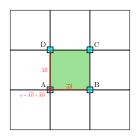
\includegraphics[scale=0.5]{./SECTIONS/TEX/ALGORITHMS/FIGURES/NormalVector}    
    \caption{Normal vector of an element}
    \label{fig:NormalVector}
  \end{figure}
  Loop over the sides of the element and check if each point satisfies
  the condition \eqref{eq:InOutSide}.
  \begin{equation}
    \label{eq:InOutSide}
    \overrightarrow{n} \cdot (\overrightarrow{AB} \wedge \overrightarrow{AP_i}) > 0
  \end{equation}
  where $\overrightarrow{n}$ is the normal vector of the element defined in
  \eqref{eq:NormaVectorElement}, $\overrightarrow{AB}$ is the array of
  the side of the element, and $\overrightarrow{AP_i}$ is the array to
  the material point measured from the initial vertex of the side. If
  it is true, for all the sides, the point is inside of the
  element, else if this condition is false in some of the sides,  the
  point it is outside and we can break the loop.  
  
  \begin{figure}
    \centering
    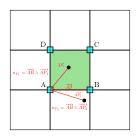
\includegraphics[scale=0.5]{./SECTIONS/TEX/ALGORITHMS/FIGURES/InOutPoint}    
    \caption{Look if the point is in our out of the element}
    \label{fig:InOutPoint}
  \end{figure}


  \item If the point is not in the same element, search in the
    neighbour elements of the initial one. In this step of the local
    algorithm, we have two chooses, the first one and the easy one to
    program is search in the elements around the initial one. The
    second one is which we have implemented in our code and consist in
    use the velocity field to predict in which element will be the
    particle. For this algorithm, this are the steps :
    \begin{enumerate}
    \item For each vertex of the element, get the direction of search
      of this vertex as the sum of the arrays of the sides that reach
      to this vertex.
      \begin{equation}
        \label{eq:VertexSeachDirection}
        \overrightarrow{n_B} = \overrightarrow{AB} + \overrightarrow{CB}
      \end{equation}
    \item For each dimension of $\overrightarrow{n_B}$, multiply it
      component by component by the velocity vector of the material
      point, like some kind of projection, if all the components of
      the resultant vector are positive we should search the material
      point in this direction, else if try in the next node.

    \item 
    \end{enumerate}

  
  
\end{enumerate}



%%% Local Variables:
%%% mode: latex
%%% TeX-master: "../../../mpm"
%%% End:



Como vemos en \cite{Tran2019d}



% Bibliography

\bibliographystyle{acm}
\bibliography{/home/migmolper2/Documentos/PHD/BIBLIOGRAFIA/library}

\end{document}

%%% Local Variables:
%%% mode: latex
%%% TeX-master: t
%%% End:


